\subsection{Growth Accounting}

It is important to note that in this paper, we treat light values and population density as a potential indicator of slums rather than there being some causal relationship. The main drivers of slum formation is likely the state of the economy and key characteristics such as the ratio between wages and rents which may in turn be connected to lights. We explore these macro relationships as well to gain more insight into any indirect effects. To begin, as the title of this subsection entails, Figure 11 shows the solow macro model growth dynamics for Kenya. Note that we have not detrended GDP and as such we see that the main reason GDP growth is not as high as it should be is due to low capital.

\begin{figure}
    \centering
    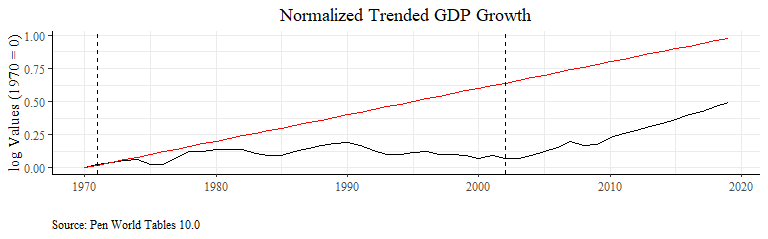
\includegraphics[scale = 0.7]{Graphics/Normalized Trended GDP Growth.png}
    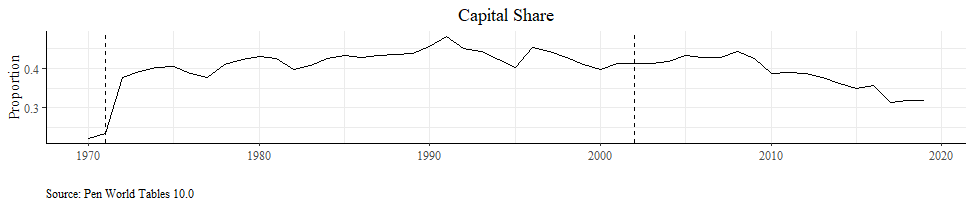
\includegraphics[scale = 0.52]{Graphics/Capital Share.png}
    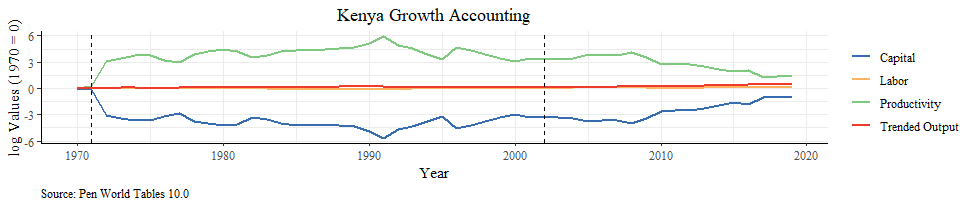
\includegraphics[scale = 0.52]{Graphics/Kenya Growth Accounting.png}
    \caption{Cobb Douglas Growth Accounting (Variable Alpha) - Kenya}
    \label{fig:KenyaGrowthAccounting}
\end{figure}

To further investigate, figure 12 shows both how aggregate average lights per square kilometer and population density per square kilometer in Kenya has fared from 2000 to 2013. As further insight into relationships between lights, population density and how a potential indirect relationship may be, the second graphic below displays the simple linear regressions of both lights and year on GDP, and GDP and year on lights. In both cases, the impact of light on GDP and GDP on light have statistically significant positive coefficients which speaks to potential confounders in terms of establishing a causal relationship between population density and light. Since we are initially only trying to estimate an indicative relationship to use as a tool to map, this confounder in the causal relationship is good because it establishes a link between slums and lights.

\begin{figure}
    \centering
    \begin{minipage}{0.45\textwidth}
    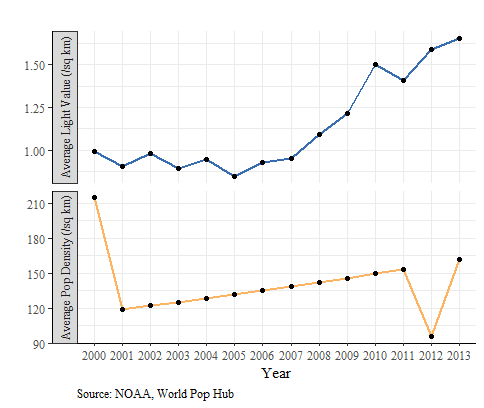
\includegraphics[scale = 0.55]{Graphics/Average lights and population density over time.png}
    \caption{Kenya, Average lights and population density over time}
    \end{minipage}
    \begin{minipage}{0.45\textwidth}
    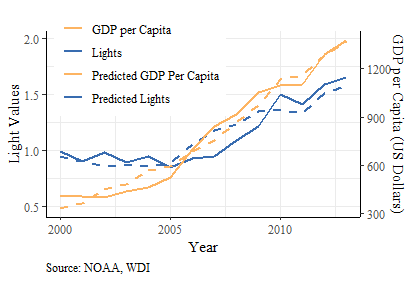
\includegraphics[scale = 0.8]{Graphics/Kenya, Average lights and GDP per Capita over time.png}
    \caption{Kenya, Average lights and GDP per Capita over time}
    \label{fig:lightpoptime}
    \end{minipage}
\end{figure}



% latex table generated in R 4.0.3 by xtable 1.8-4 package
% Mon Mar 20 00:52:26 2023
\begin{table}[ht]
\centering
\caption{Correlation Plot (GDP is per capita)}
\begin{tabular}{r|rrrrr}
  \hline\hline
 & Year & GDP & Pop Density & Lights & Detrended GDP \\ 
  \hline
Year & 1.00 & 0.97 & -0.12 & 0.85 & 0.98 \\ 
  GDP & 0.97 & 1.00 & -0.01 & 0.91 & 0.99 \\ 
  Pop Density & -0.12 & -0.01 & 1.00 & 0.05 & -0.02 \\ 
  Lights& 0.85 & 0.91 & 0.05 & 1.00 & 0.85 \\ 
  Detrended GDP & 0.98 & 0.99 & -0.02 & 0.85 & 1.00 \\ 
   \hline 
\end{tabular}
\end{table}